\documentclass[../main.tex]{subfile}
\graphicspath{{\subfix{../images}}}
\begin{document}

\subsection{卷积层和特征图}

考虑流行的七层架构\cite{alexnet, zfnet}。前五层是卷积层,其中一些接着池化层。这些池化层也可以被认为是 "卷积",因为它们使用的是滑动窗口。最后两层是全连接的,以$N$-way softmax作为输出,其中$N$是类别的数量。

上述的深度网络需要一个固定的图像大小。然而,我们注意到,对固定尺寸的要求只是由于全连接层需要固定长度的向量作为输入。另一方面,卷积层接受任意大小的输入。卷积层使用滑动卷积核,其输出与输入的长宽比大致相同。这些输出被称为特征图[1]--它们不仅涉及反应的强度,而且还涉及它们的空间位置。

在图\ref{fig:fig2}中,我们可视化了一些特征图。它们是由$\text{conv}_5$层的一些卷积核生成的。图\ref{fig:fig2}(c)显示了ImageNet数据集中这些卷积核最强的激活图像。我们看到一个卷积核可以被一些语义内容所激活。例如,第55个卷积核(图\ref{fig:fig2},左下)被圆形激活最多;第66个卷积核(图\ref{fig:fig2},右上)被$\wedge $形激活最多;第118个卷积核(图\ref{fig:fig2},右下)被$\vee $形激活最多。输入图像中的这些形状(图\ref{fig:fig2}(a))激活了相应位置的特征图(图\ref{fig:fig2}中的箭头)。

值得注意的是,我们生成图\ref{fig:fig2}中的特征图时没有固定输入尺寸。这些由深度卷积层生成的特征图类似于传统方法中的特征图[27], [28]。在这些方法中,SIFT向量[29]或图像斑块[28]被密集提取,然后进行编码,例如,通过向量量化[16]、[15]、[30]、稀疏编码[17]、[18]或Fisher内核[19]。这些编码后的特征由特征图组成,然后通过词袋(BoW)\cite{bow}或空间金字塔\cite{sp1, sp2}进行汇集。类似地,深度卷积特征也可以用类似的方式进行汇集。

\subsection{空间金字塔池化层}

卷积层接受任意大小的输入,但它们产生的输出是大小可变的。分类器(SVM/softmax)或全连接层需要固定长度的向量。这种向量可以通过将特征汇集在一起的词袋(BoW)方法\cite{bow}产生。空间金字塔集合\cite{sp1, sp2}改进了BoW,因为它可以通过在局部空间仓中集合来保持空间信息。这些空间仓的大小与图像大小成正比,因此无论图像大小如何,仓的数量是固定的。这与之前的深度网络\cite{alexnet}中的滑动窗池化形成对比,后者的滑动窗数量取决于输入大小。


\begin{figure}[htb]
    \centering
    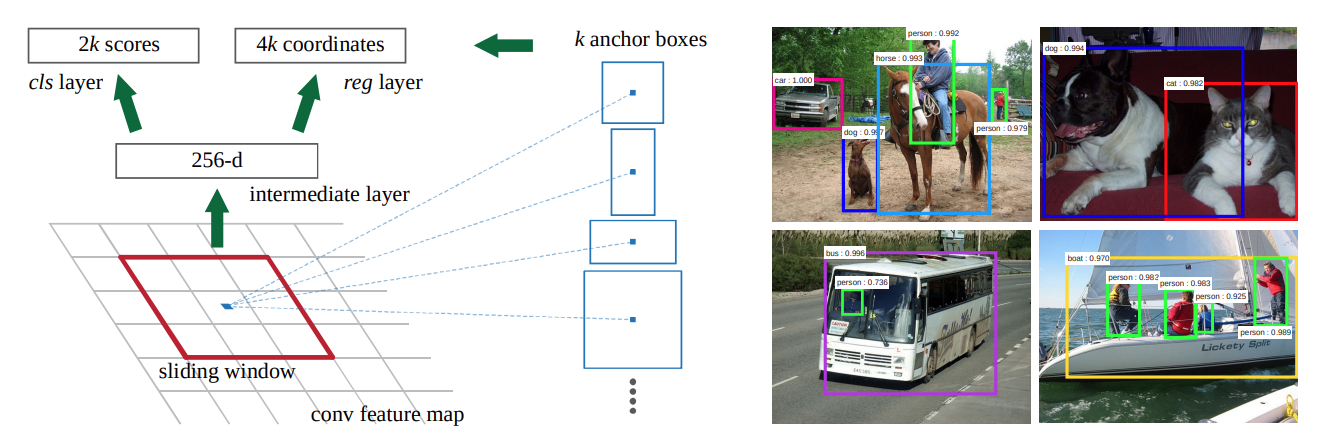
\includegraphics[width=\textwidth]{fig3.png}
    \caption{一个具有\textbf{空间金字塔池化层}的网络结构。这里256是最后一个卷积层$\text{conv5}_5$的卷积核数量。}
    \label{fig:fig3}
\end{figure}

为了对任意大小的图像采用深度网络,我们用空间金字塔池化层取代了最后一个池化层(例如在最后一个卷积层之后的$\text{pool}_5$)。图\ref{fig:fig3}说明了我们的方法。在每个空间仓中,我们汇集每个卷积核的响应(在本文中我们使用最大池化)。空间金字塔池化的输出是一个$kM$维向量,仓的数量表示为$M$($k$是最后一个卷积层中的卷积核数量)。固定维度的向量是全连接层的输入。

通过空间金字塔集合,输入图像可以是任何尺寸。这不仅允许任意的长宽比,还允许任意的比例。我们可以将输入图像的大小调整为任何比例(例如,$\min\left(w, h\right) = 180,224,\ldots$),并应用相同的深度网络。当输入图像处于不同尺度时,网络(具有相同的卷积核大小)将提取不同尺度的特征。尺度在传统方法中起着重要的作用,例如,SIFT向量通常是在多个尺度上提取的[29],[27](由斑块和高斯卷积核的大小决定)。我们将表明,尺度对深度网络的准确性也很重要。

有趣的是,最粗糙的金字塔层仅有一个覆盖整个图像的单仓。这实际上是一种“全局池化”操作,在几个同时进行的工作中也有研究。在[31]、[32]中,全局平均池化被用来减少模型的大小,也减少了过拟合;在[33]中,全局平均池化被用在所有$fc$层之后的测试阶段,以提高准确性;在[34]中,全局最大池化被用于弱监督的物体识别。全局池化操作对应于传统的Bag-of-Words方法。

\subsection{网络训练}

理论上,上述网络结构可以用标准的反向传播算法[1]来训练,而不考虑输入图像的大小。但在实践中,GPU的实现(如cuda-convnet[3]和Caffe[35])最好是在固定的输入图像上运行。接下来我们将介绍我们的训练方案,该方案利用了这些GPU实现,同时仍然保留了空间金字塔池的行为。

\subsubsection*{大一大小训练}

和以前的工作一样,我们首先考虑一个网络从图像中获取固定尺寸的输入($224\times 224$)。裁剪的目的是为了增加数据。对于一个给定尺寸的图像,我们可以预先计算出空间金字塔池化所需的仓尺寸。考虑$\text{conv}_5$之后的特征图,其大小为$a\times a$(例如$13\times 13$)。对于一个有$n\times n$个仓金字塔层级,我们将这个池化层级实现为滑动窗口池化,其中窗口大小$win=\lceil a/n \rceil $,$stride = \lfloor a/n \rfloor$,$\lceil \cdot \rceil $和$\lfloor \cdot \rfloor$表示向上取整和向下取整的操作。通过一个$l$级的金字塔,我们实现了$l$个这样的层。下一个全连接的层($\text{fc}_6$)将把$l$个输出连接起来。图\ref{fig:fig4}显示了\textit{cuda-convnet}风格\cite{alexnet}的3级金字塔池化($3\times 3, 2\times 2, 1\times 1$)的配置实例。

\begin{figure}[htb]
    \centering
    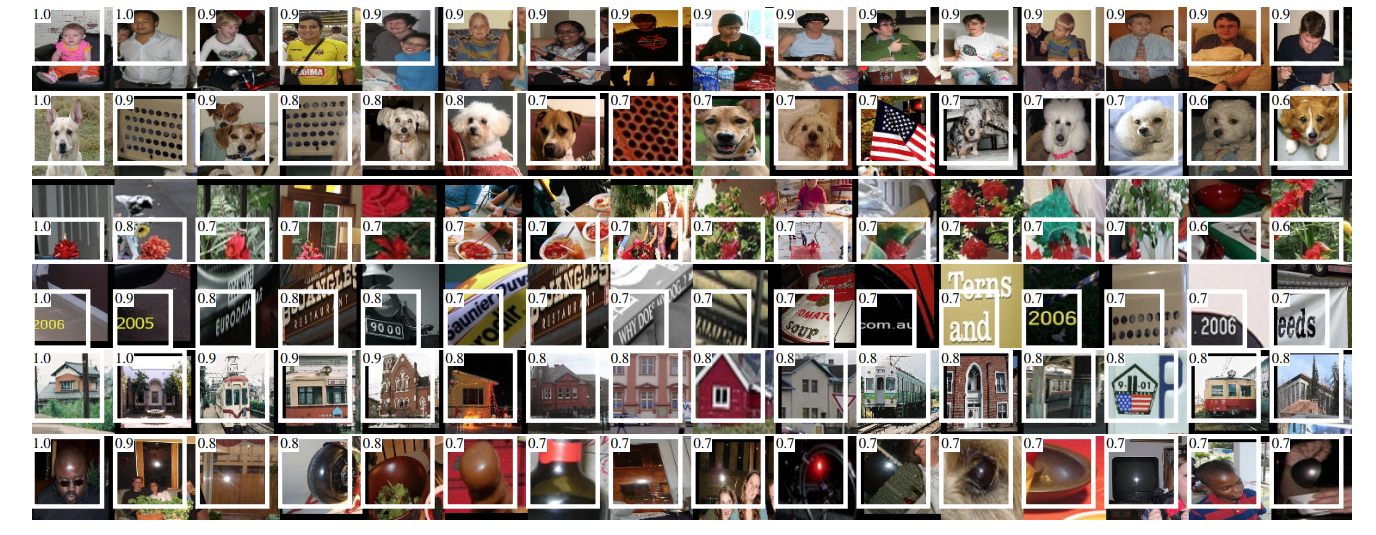
\includegraphics[width=\textwidth]{fig4.png}
    \caption{一个\textit{cuda-convnet}风格\cite{alexnet}的3级金字塔池的例子。这里sizeX是池化窗口的大小。这个配置是针对一个$\text{conv}_5$的特征图大小为$13\times 13$的网络,所以$\text{pool}_{3\times 3}, \text{pool}_{2\times 2}$和$\text{pool}_{1\times 1}$层将分别有$3\times 3, 2\times 2$和$1\times 1$个仓。}
    \label{fig:fig4}
\end{figure}

我们进行单一尺度训练的主要目的是为了实现多级池化行为。实验表明,这是提高准确率的一个原因。

\subsubsection*{多大小训练}

我们的拥有SPP的网络预计将应用于任何尺寸的图像。为了解决训练中不同图像尺寸的问题,我们考虑一组预定义的尺寸。我们考虑两种尺寸。$180\times 180$,以及$224\times 224$。我们没有裁剪一个较小的$180\times 180$区域,而是将上述$224\times 224$区域的大小调整为$180\times 180$。因此,两种比例的区域只在分辨率上有区别,而在内容/布局上没有区别。为了让网络接受$180\times 180$的输入,我们实现了另一个固定大小的输入($180\times 180$)网络。在这种情况下,$conv5$之后的特征图大小为$a\times a=10\times 10$。然后我们仍然使用$win=\lceil a/n \rceil $和$stride = \lfloor a/n \rfloor$来实现每个金字塔池化的层级。这个180网络的空间金字塔池化层的输出与224网络的固定长度相同。因此,这个180网络的每一层的参数与224网络的参数完全相同。换句话说,在训练过程中,我们通过两个共享参数的固定尺寸网络来实现变化输入尺寸的SPP网络。

为了减少从一个网络(如224)切换到另一个网络(如180)的开销,我们在一个网络上训练每个完整的纪元,然后在下一个完整的纪元切换到另一个网络(保持所有权重)。这样反复进行。在实验中,我们发现这种多规模训练的收敛率与上述单规模训练相似。

我们的多规模训练的主要目的是模拟不同的输入尺寸,同时仍然利用现有的经过优化的固定尺寸实现。除了上述两个尺寸的实现,我们还测试了一个使用$s\times s$作为输入的变体,其中$s$是在每个历时中通过从$\left[ 180, 224\right]$中随机均匀取样得到。我们在实验部分报告了这些变体的结果。

请注意,上述单/多尺寸的解决方案仅用于训练。在测试阶段,在任何尺寸的图像上应用SPP-net都是直接的。

\end{document}